\documentclass[../main.tex]{subfiles}
\graphicspath{{\subfix{../images/}}}
\begin{document}

  A seguir, serão apresentados os resultados preliminares e os experimentos realizados com o Caramelo. Este refere-se aos testes mencionados na seção \ref{sec:method_results_analysis} enquanto aquele refere-se aos resultados obtidos com as funcionalidades básicas do robô: capacidade de movimentação a partir do modelo cinemático e capacidade de controle da orientação do corpo com o controlador de angulação.
  
  \subsection{Resultados preliminares}

  Os primeiros testes realizados com o protótipo foram relacionados à movimentação do corpo a partir do modelo cinemático. Foi observado que o sistema não só é capaz de realizar a cinemática de cada uma das pernas individualmente como também do seu corpo em todos os 6 graus de liberdade (translações em $x$, $y$ e $z$ e rotações em $roll$, $pitch$ e $yaw$). A figura \ref{fig:moving_body} ilustra o movimento do corpo do robô em cada um desses graus de liberdade.

  \begin{figure}[!htb]
    \centering
    \caption{Movimentação do corpo do robô.}
    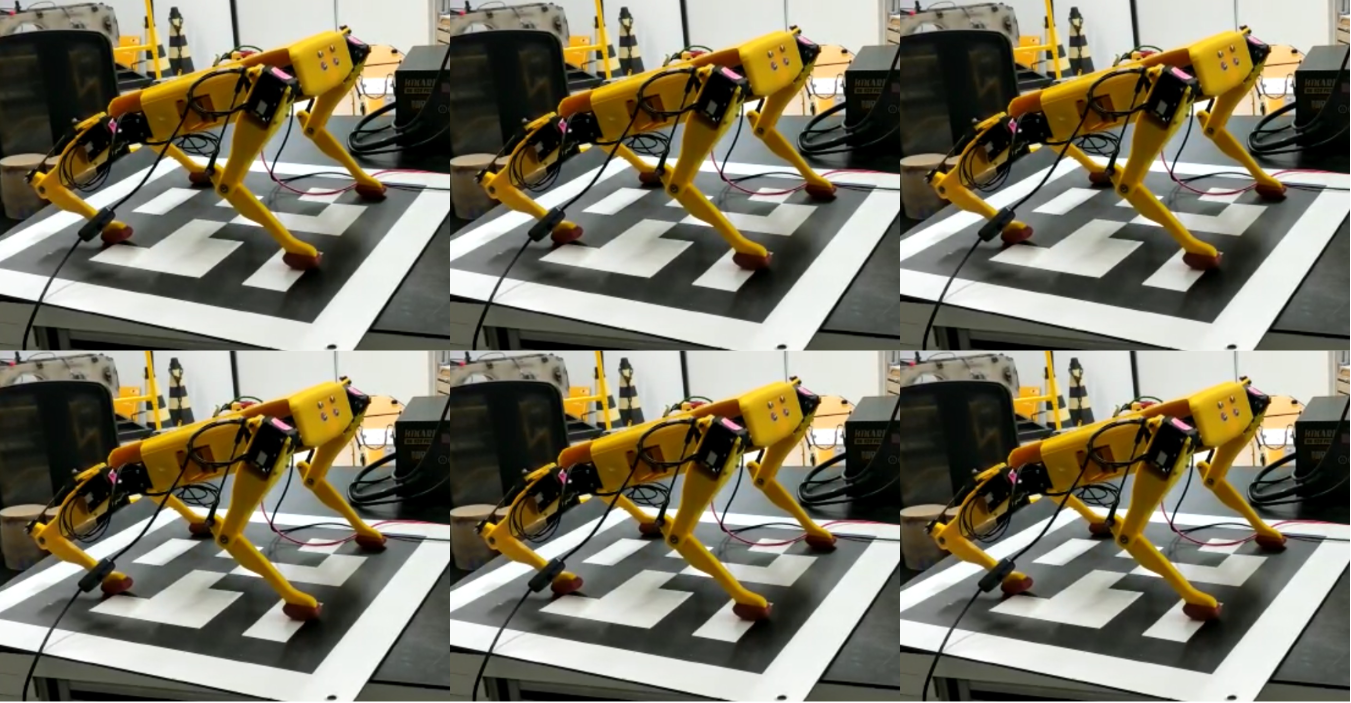
\includegraphics[width=0.48\textwidth]{moving_body.png}
    
    Fonte: autores.
    \label{fig:moving_body}
  \end{figure}

  Do mesmo modo, os gráficos da figura \ref{fig:grafico_controlling} ilustram o comportamento do sistema à variação dos \textit{setpoints} de orientação em \textit{roll} (gráfico superior) e em \textit{pitch} (gráfico inferior) para o corpo do robô, a partir da aplicação de diversos degraus (curvas em azul). Nota-se que o protótipo é capaz de se adaptar rapidamente aos novos valores desejados de orientação simultaneamente em ambos os eixos.

  \begin{figure}[!htb]
    \centering
    \caption{Respostas dos controles de angulação}
    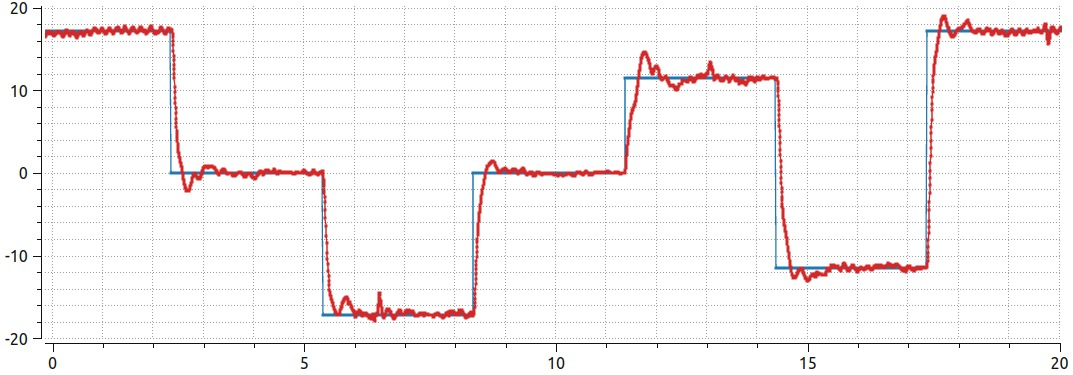
\includegraphics[width=0.48\textwidth]{grafico_controlling_X.png}
    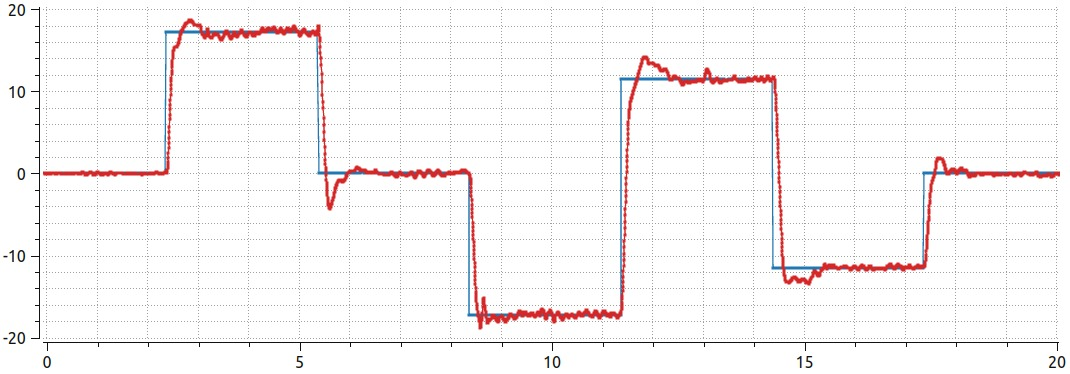
\includegraphics[width=0.48\textwidth]{grafico_controlling_Y.png}
    
    Fonte: autores
    \label{fig:grafico_controlling}
  \end{figure}

  \subsection{Experimentos}
  Em seguida, serão apresentados os resultados dos experimentos descritos na seção \ref{sec:method_results_analysis}.

  \subsubsection{Análise de trajetória}
  Durante este experimento, o objetivo foi analisar o tempo real de execução da trajetória, as coordenadas finais $(x_f, y_f)$ da pata e a altura máxima $z_{max}$ atingida durante o passo, comparando-os com os valores esperados para cada um desses parâmetros. A tabela \ref{tab:trajetoria} mostra as médias encontradas para cada um desses parâmetros durante a realização dos testes.

  \begin{table}[!htb]
    \caption{Resultados do experimento da trajetória da pata.}
    \centering
    \begin{tabular}{ccc}
      \hline
                            & 1         & 2        \\
      \hline
      $\bar{tempo}$ (s)          & 0.569965  & 0.576984 \\
      \hline
      $\sigma_{tempo}$            & 0.058441  & 0.077332 \\
      \hline
      $\bar{x}_{final}$ (m)     & 0.050344  & 0.030237 \\
      \hline
      $\sigma_{x_{final}}$ (m)  & 0.000104  & 0.000134 \\
      \hline
      $\bar{y}_{final}$ (m)     & 0.029242  & 0.049143 \\      
      \hline
      $\sigma_{y_{final}}$ (m)  & 0.000128  & 0.000095 \\      
      \hline
      $\bar{z}_{max}$ (m)       & 0.047568  & 0.046162 \\      
      \hline
      $\sigma_{z_{max}}$    & 0.000278  & 0.005562 \\
      \hline   
    \end{tabular}

    Fonte: autores.
    \label{tab:trajetoria}
  \end{table}

  Inicialmente, foram realizados dois testes de t-Student para amostras independentes, o primeiro relacionando o tempo de execução da trajetória nos experimentos 1 e 2, e o segundo relacionando a altura máxima alcançada, com o intuito de verificar se os resultados se alteram para diferentes valores $(x, y)$ desejados. O resultado da análise de t-Student traz um $p_{valor}$ de aproximadamente $0.6931$, em se tratando de tempo, e de $0.1722$ para a altura máxima alcançada durante o passo. Ambos os valores encontrados são superiores a $0.05$, o que mostra que, para uma confiabilidade de $95\%$, não há uma diferença significativa entre as médias em cada experimento, o que significa que diferentes comandos de trajetórias em $(x, y)$ não interferem nos resultados de tempo e altura máxima do passo.
  
  Os gráficos da figura \ref{fig:grafico_trajetoria_xyz} representam um dos testes realizados para o primeiro caso ($x=0.05m$, $y=0.03m$), sendo os gráficos superiores esquerdo e direito correspondentes à trajetória em $x$ e $y$ respectivamente, e o gráfico inferior correspondente à trajetória em $z$ (altura do passo). Nota-se que, como esperado pela análise da tabela \ref{tab:trajetoria}, há um atraso na execução da trajetória (neste caso específico de aproximadamente $54ms$) e a altura máxima alcançada é levemente inferior à desejada (alcançando neste caso um valor próximo a $0.0476m$).

  \begin{figure}[!htb]
    \centering
    \caption{Trajetórias realizadas pelas patas.}
    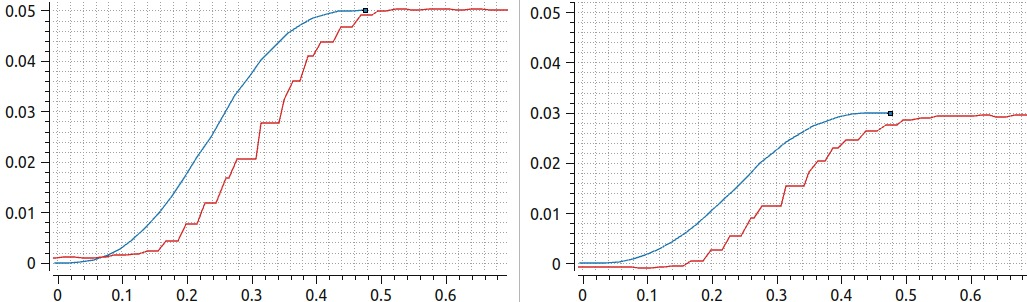
\includegraphics[width=0.48\textwidth]{grafico_trajetoria_xy.png}
    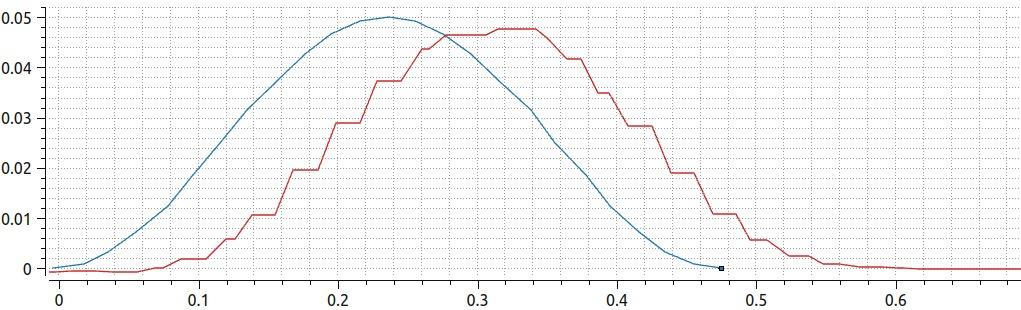
\includegraphics[width=0.48\textwidth]{grafico_trajetoria_z.png}
    
    Fonte: autores.
    \label{fig:grafico_trajetoria_xyz}
  \end{figure}

  \subsubsection{Controle de velocidade}
  Durante os testes de controle de velocidade foi observada uma caminhada eficiente em ambos os terrenos, porém, mais linear e com menor trepidação em terrenos regulares do que em terrenos irregulares. Por meio dos dados coletados, foram extraídas as informações da velocidade média da caminhada para cada teste, oscilação máxima de rotação do corpo em \textit{roll} e \textit{pitch} e os respectivos desvios padrões, apresentados na Tabela \ref{tab:vel_stab}. Assim, foi observado que o robô se aproximou mais vezes da velocidade solicitada no terreno regular combinado ao controle de rotação, enquanto que no irregular, o teste com controle de rotação ativo apresentou uma velocidade média inferior e baixa consistência nos dados. A diferença percebida entre a velocidade solicitada e a inferida é justificada pelo acúmulo de erro nas coordenadas finais $(x_f, y_f)$ das patas a cada passo. Ou seja, quando levado em consideração o próprio peso do robô, o sistema de controle não é capaz de seguir fielmente a trajetória do passo.

  \begin{table}[!htb]
    \caption{Resultados do experimento do controlde de velocidade.}
    \centering
    \begin{tabular}{ccccc}
      \hline
      & 1 & 2 & 3 & 4 \\ \hline
      Ter. & Reg. & Reg. & Irreg. & Irreg. \\ \hline
      \begin{tabular}[c]{@{}c@{}}C. R.\end{tabular} & Não & Sim & Não & Sim \\ \hline
      \begin{tabular}[c]{@{}c@{}}Vel. \\ (cm/s) \end{tabular} &   2.92   &  3.33  &   2.97   & 2.77  \\ \hline
      \begin{tabular}[c]{@{}c@{}} $\sigma_{Vel}$  \\ (cm/s) \end{tabular} & 0.135 & 0.079 & 0.197 & 0.241 \\ \hline
      \begin{tabular}[c]{@{}c@{}} $\Delta_{Roll}$ \end{tabular} & 12.54\degree & 8.74\degree & 13.90\degree & 12.17\degree \\\hline
      \begin{tabular}[c]{@{}c@{}} $\sigma_{Roll}$ \end{tabular}  & 2.42\degree & 2.14\degree & 1.80\degree & 3.27\degree \\ \hline
      \begin{tabular}[c]{@{}c@{}} $\Delta_{Pitch}$ \end{tabular} & 11.46\degree & 8.29\degree & 15.19\degree & 13.18\degree \\ \hline
      \begin{tabular}[c]{@{}c@{}} $\sigma_{Pitch}$ \end{tabular}  & 1.83\degree & 2.39\degree & 1.44\degree & 2.94\degree \\ \hline

    \end{tabular}
    Fonte: autores.
    \label{tab:vel_stab}
  \end{table}

  Ainda na Tabela \ref{tab:vel_stab}, foi observado que a menor oscilação em \textit{roll} e em \textit{pitch} ocorreu no terreno regular utilizando o controle de rotação, enquanto que a maior oscilação ocorreu nas condições opostas (teste 3). A fim de avaliar se o controle de rotação implementado contribuiu na estabilidade da caminhada, foi utilizado o teste t-Student para amostras independentes, considerando um nível de confiança de 95\%. O teste de t-Student foi feito comparando os testes 1 e 2 (mostrados na tabela), e os testes 3 e 4, ou seja. O resultado desta análise mostra que para terrenos planos, a hipótese nula de que o controle de rotação não influencia na estabilidade do robô pode ser rejeitada, pois o p-valor se mostrou menor que $0,05$. Ou seja, neste caso, o controle de rotação ajudou a estabilizar o corpo do robô. Entretanto, para terrenos irregulares, o uso do controlador não ocasionou mudanças significativas na estabilidade do robô, dado o p-valor de $0,0778$. Logo, para terrenos irregulares, o controlador de rotação não se mostrou eficiente para estabilizar o corpo do robô. 
    
  \subsubsection{Plano inclinado}
  Durante este experimento, contatou-se que o robô possui a habilidade de andar por terrenos com $5,336\degree$ de inclinação, figura \ref{fig:tests3-4}. 

  \subsubsection{Superação de obstáculos}
  O último experimento constatou que o robô é capaz de ultrapassar pequenos obstáculos. Para isso, foram considerados degraus de três diferentes alturas: 2, 4 e 5 $cm$ (ver figura \ref{fig:tests3-4}). O robô foi capaz de superar degraus de 2 e 4 $cm$, porém falhou ao tentar subir um de 5 $cm$.

  \begin{figure}[!htb]
    \centering
    \caption{Fotos do robô no teste da rampa e do degrau.}
    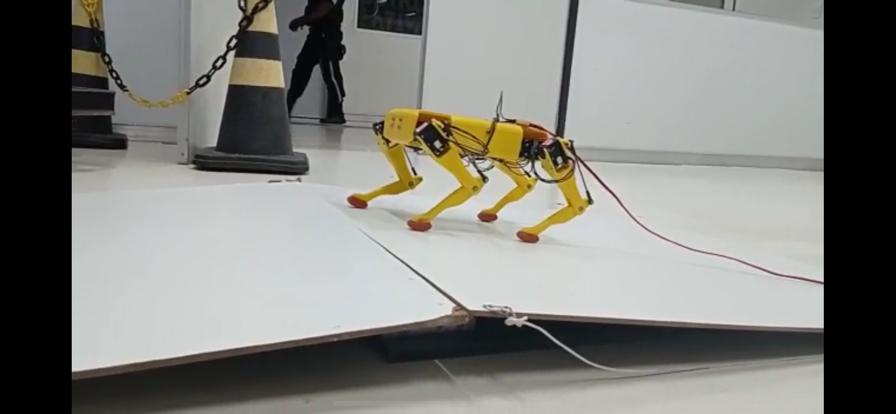
\includegraphics[width=0.48\textwidth]{ramp_test.jpeg}
    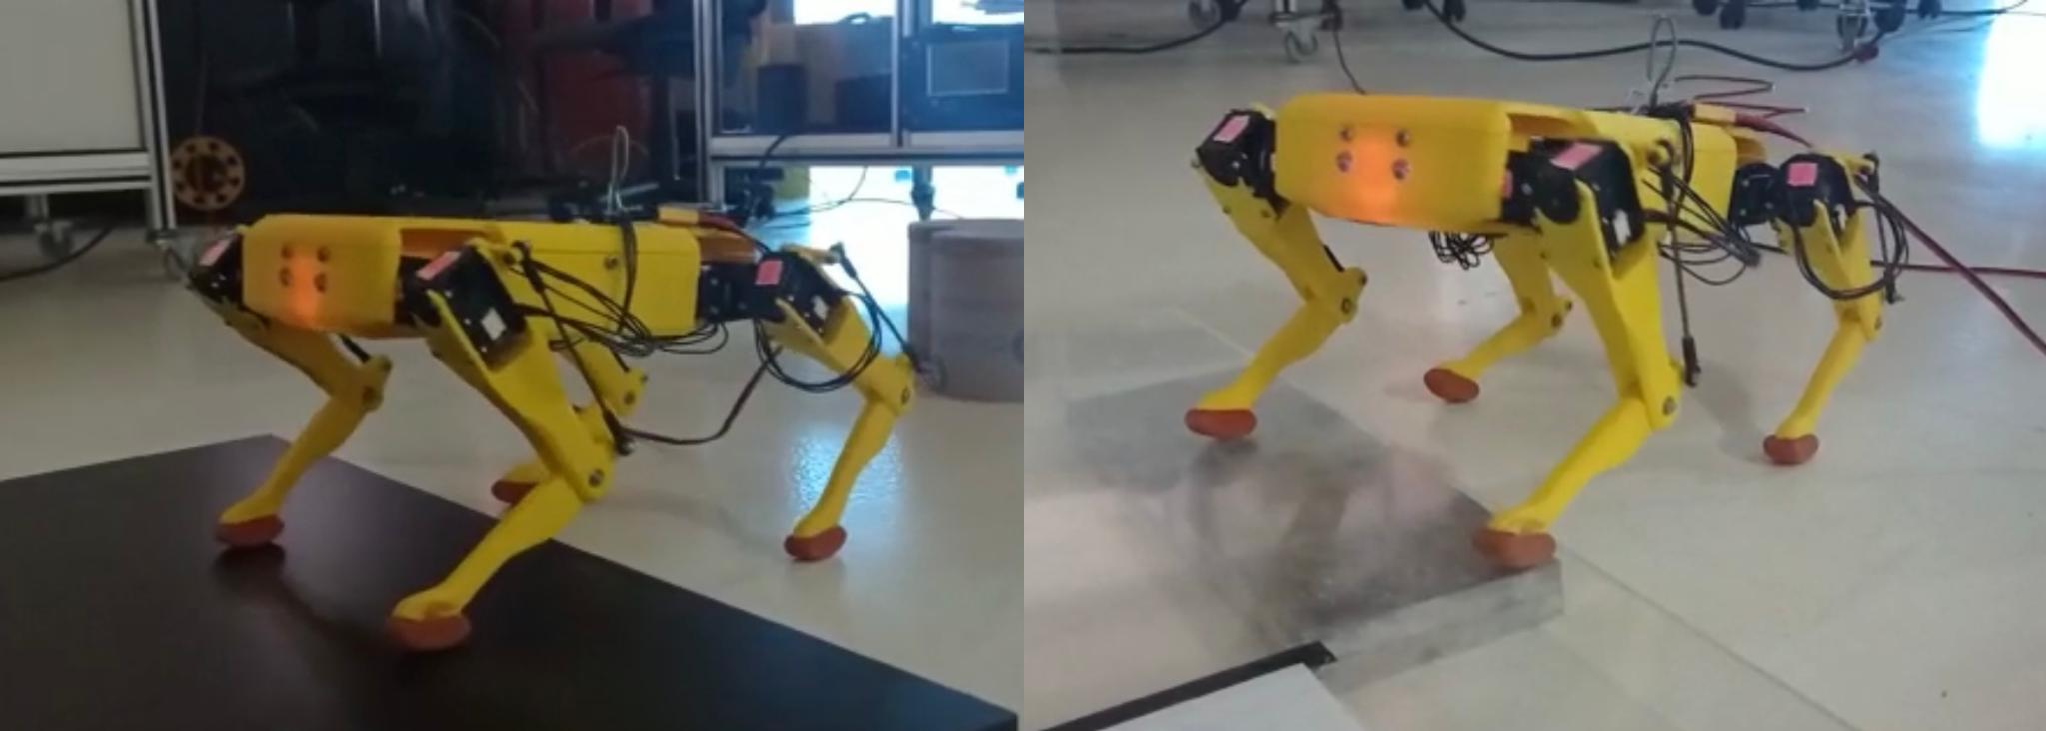
\includegraphics[width=0.48\textwidth]{test4.png}

    Fonte: autores
    \label{fig:tests3-4}
  \end{figure}

\end{document}